%%%%%%%%%%%%%%%%%%%%%%%%%%%%%%%%%%%%%%%%%%%%%%%%%%%%%%%%%%%%%%%%%%%%%%%%

%%% Manuscript file by Robert Haase, license CC-BY 4.0
%%% https://github.com/haesleinhuepf/git-bob-manuscript
%%%
%%% Based on Ricardo Henriques bioRxiv template, license CC-BY 4.0
%%% https://www.overleaf.com/latex/templates/henriqueslab-biorxiv-template/nyprsybwffws
%%% https://creativecommons.org/licenses/by/4.0/deed.en 

%%%%%%%%%%%%%%%%%%%%%%%%%%%%%%%%%%%%%%%%%%%%%%%%%%%%%%%%%%%%%%%%%%%%%%%%

\documentclass[times, twoside]{zHenriquesLab-StyleBioRxiv}
\usepackage{blindtext}

% Please give the surname of the lead author for the running footer
\leadauthor{Haase} 

\begin{document}

\title{Towards Transparency and Knowledge Exchange in AI-assisted Data Analysis Code Generation}
\shorttitle{Towards Transparency and Knowledge Exchange in AI-assisted Data Analysis Code Generation}

% Use letters for affiliations, numbers to show equal authorship (if applicable) and to indicate the corresponding author
\author[1,2,3,\Letter]{Robert Haase}

\affil[1]{Data Science Center, Leipzig University, Humboldtstra{\ss}e 25, 04105 Leipzig, Germany}
\affil[2]{Center for Scalable Data Analytics and Artificial Intelligence (ScaDS.AI) Dresden / Leipzig}
\affil[3]{National Research Data Infrastructure for Microscopy and BioImage Analysis, NFDI4BioImage}

\maketitle

%TC:break Abstract
%the command above serves to have a word count for the abstract
\begin{abstract}

The integration of Large Language Models (LLMs) in scientific research presents both opportunities and challenges for scientists. Key challenges include ensuring transparency in artificial intelligence (AI)-generated content and facilitating efficient knowledge exchange among researchers. These issues arise from the intransparent nature of AI-driven code generation and the informal sharing of AI insights, which may hinder reproducibility and collaboration. This paper introduces git-bob, an innovative AI-assistant designed to address these challenges by fostering an interactive and transparent collaboration platform within GitHub and GitLab. While enabling seamless dialogue between mutliple humans and multiple LLMs in one thread, git-bob ensures that AI-generated contributions are transparent and reproducible. Moreover, it supports collaborative knowledge exchange, enhancing the interdisciplinary dialogue necessary for cutting-edge research. The open-source nature of git-bob further promotes accessibility and customization, positioning it as a vital tool in employing LLMs responsibly and effectively within scientific communities.

\end {abstract}
%TC:break main
%the command above serves to have a word count for the abstract

\begin{keywords}
Data Analysis, LLM, Code Generation
\end{keywords}

\begin{corrauthor}
robert.haase@uni-leipzig.de, ORCID: 0000-0001-5949-2327
\end{corrauthor}



\section*{Introduction}

Generative artificial intelligence (AI) and Large Language Models (LLMs) in particular are changing the way we do data science. Most prominently, scientists use the technology for interacting with scientific data \cite{Royer2023}, answer data analysis questions \cite{Lai2022DS1000, lei2024bioimage}, generate data analysis code \cite{Royer2024, benchmark_llm_bia, chen2021evaluating}, and [re-]write scientific manuscripts \cite{lu2024aiscientist}. Unfortunately, the prompts sent to LLMs are commonly not conserved, and thus, at the time of publication, it might be hard to differentiate human-made and AI-generated parts of the scientific work. A professional peer-review system, for documenting how LLM-generated code was prompted for, and which human reviewed it, is not established in contemporary scientific culture. However, such systems do exist for collaborative code editing involving multiple humans. For example, the online platform github.com is well-established in the open-source software community for discussing issues and potential solutions, building code together, and for peer-reviewing contents. As it was shown before that LLMs can solve real-world GitHub issues \cite{jimenez2024swebenchlanguagemodelsresolve}, developing an AI-assistant that interacts with humans directly within the Github platform is the obvious next step. I am presenting git-bob, an implementation of an LLM-based AI-assistant that can respond to GitHub issues, discuss potential solutions with humans iteratively, write code for them, and submit it as pull-request to be reviewed by humans. It is technically similar to various online services for data analysis such as the OpenAI ChatGPT Data Analyst or Github Copilot Workflows, with three major differences: 1) Multiple humans can interact with git-bob in one communication thread. This allows bringing together domain specialists, such as life scientists, data-analysts and the AI-assistant in one discussion, stimulating knowledge exchange on how to interact properly with the AI-assistant. 2) Discussions with git-bob and resulting code modifications are conserved in an online-platform that others can read and follow, making the interaction with the AI-assistant fully transparent, and 3) git-bob is open-source. Other developers can read its built-in system prompts and modify them to their needs. Git-bob's source code is available online: \url{https://github.com/haesleinhuepf/git-bob}.

%%%%%%%%%%%%%%%%%%%%%%%%%%%%%%%%%%%%%%%%%%%%%%%%%%%%%%%%%%%%%%%%%%%%%%%%

\begin{figure}[h]
\centering
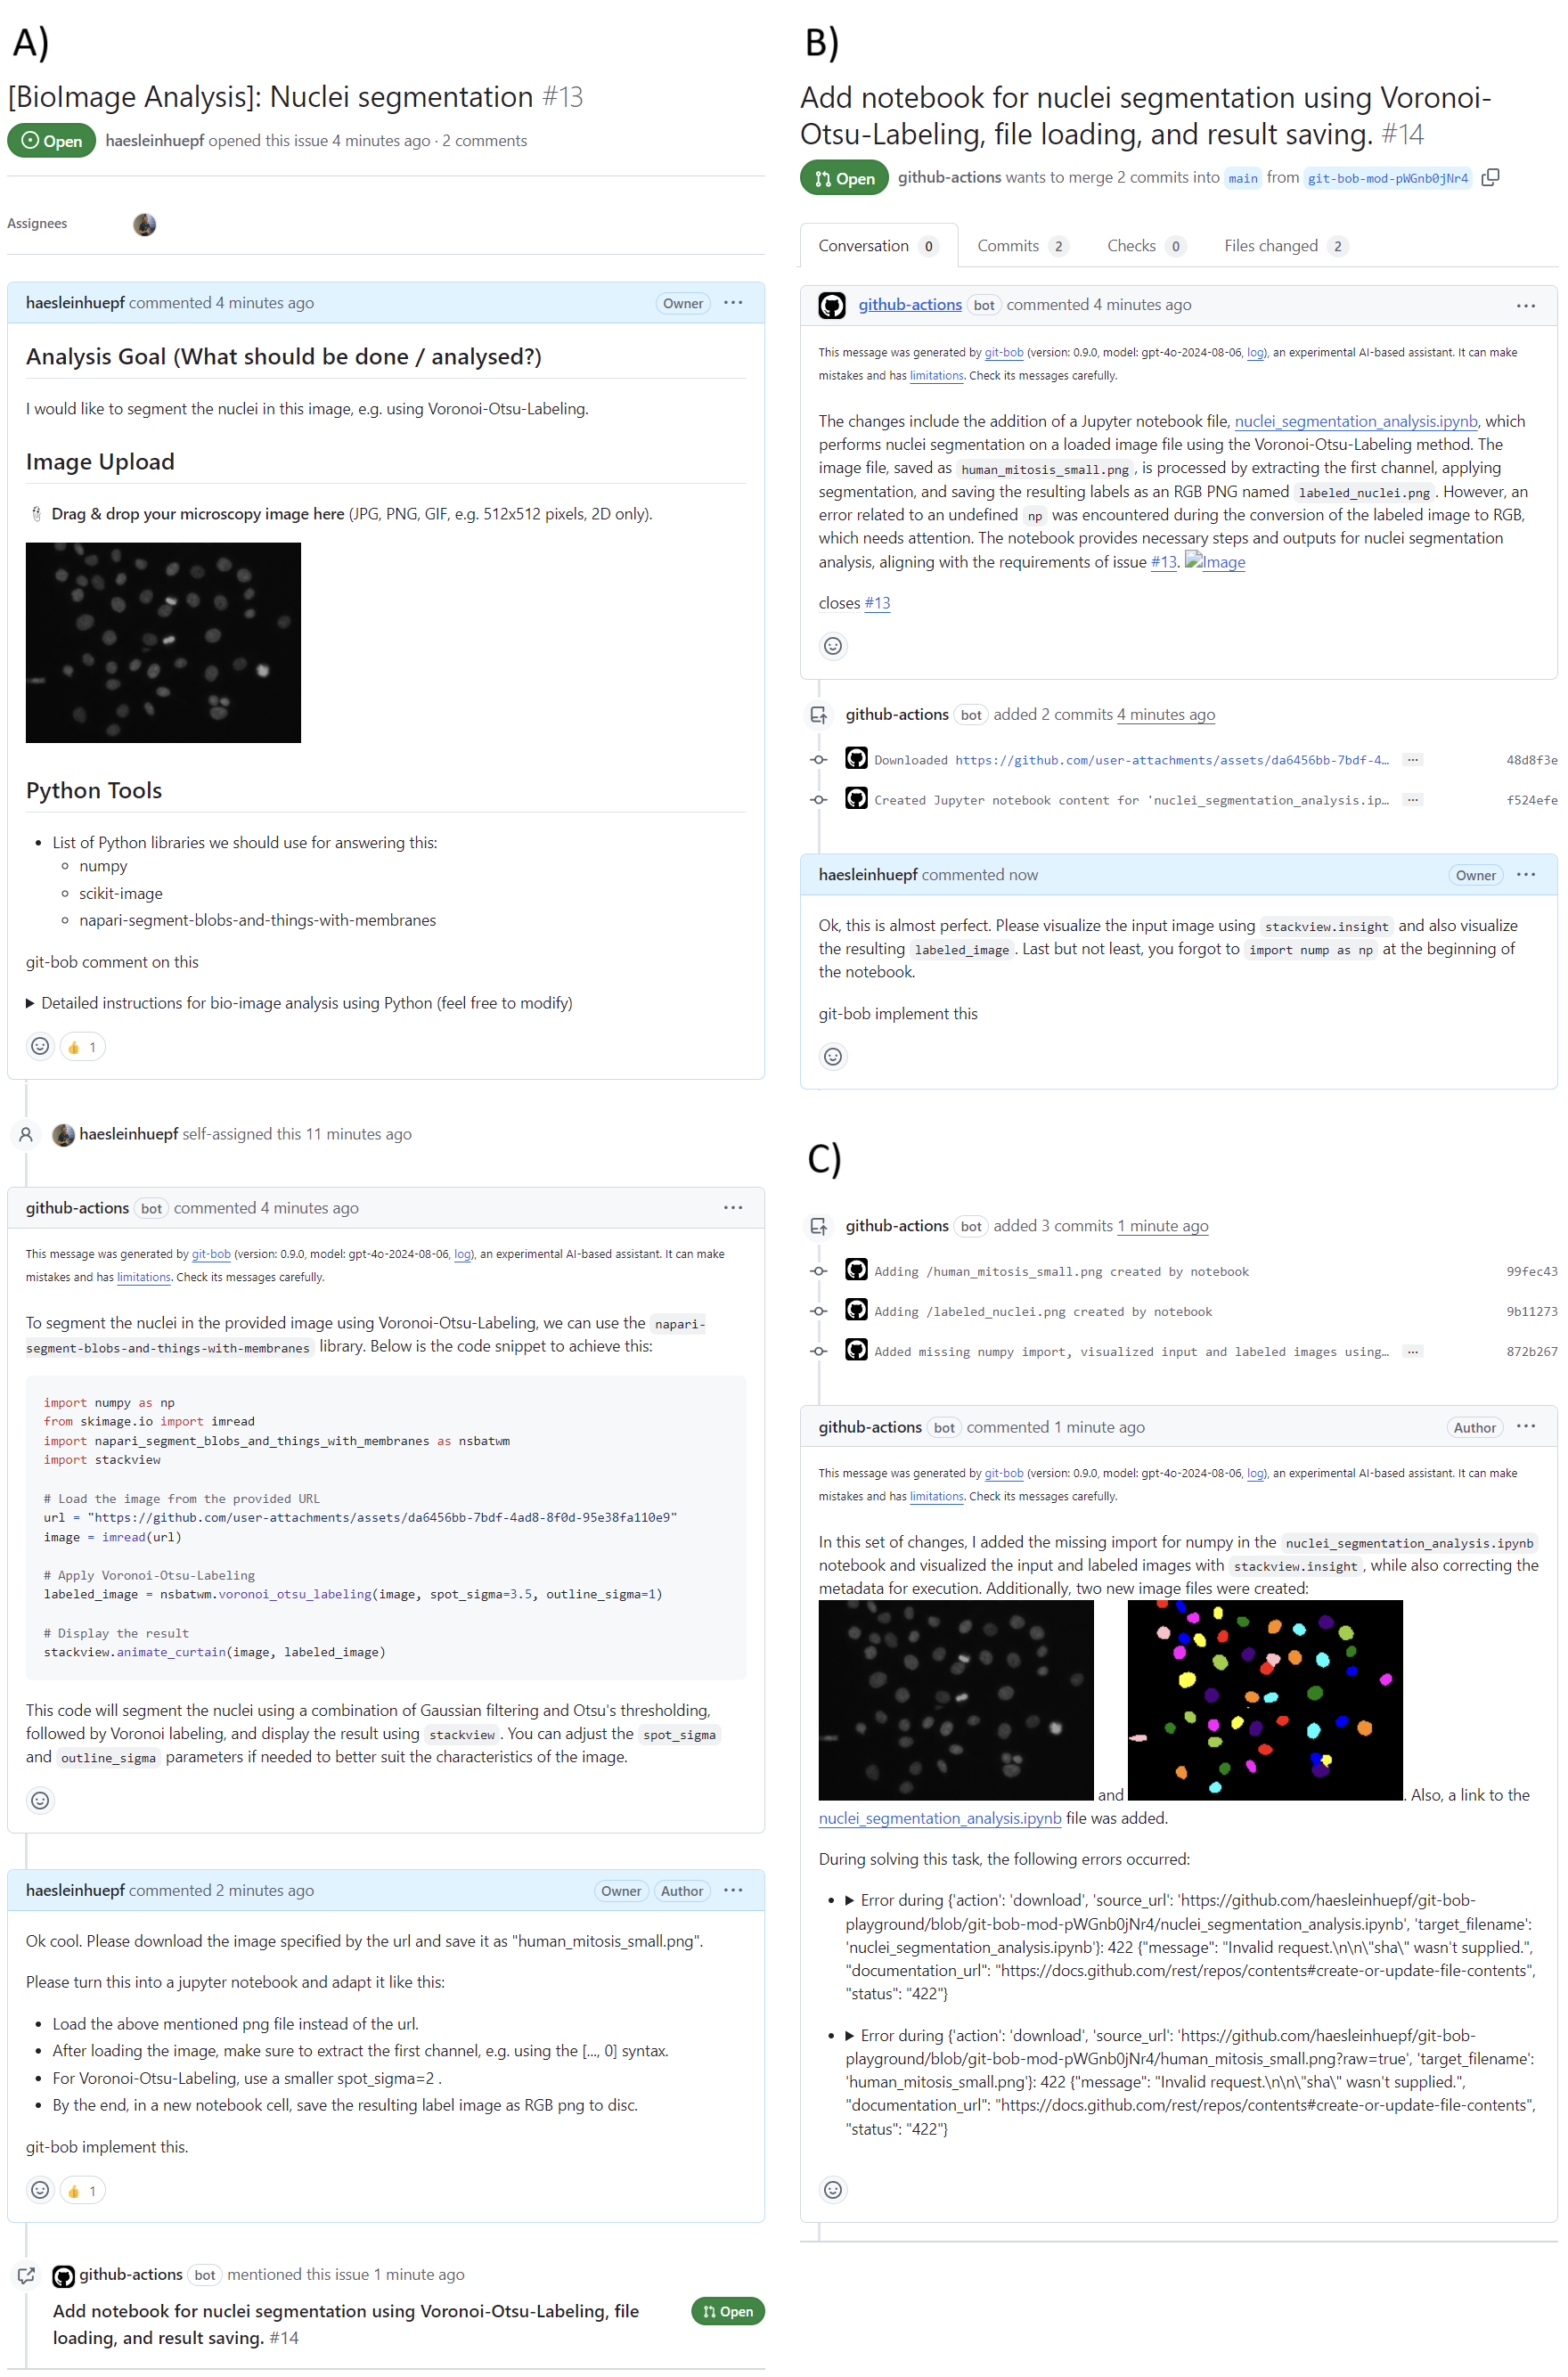
\includegraphics[width=0.5\textwidth]{example_interaction.png}
\caption{Schematic view of the interaction with git-bob: In one discussion thread, multiple humans (H) can interact with the AI-assistant which is installed in Github or Gitlab Continuous Integration (CI) infrastructure. Depending on how it is triggered, the AI-assistant may use LLMs from multiple LLM service providers in the background.
\newline
\newline
}
\label{fig:example_interaction}
\end{figure}

\section*{Features and limitations} 

A schematic workflow involving git-bob is drawn in Figure \ref{fig:example_interaction}: a domain expert opens an issue, a kind of discussion thread, on a repository on github.com, where git-bob is installed. A repository member can then add more information to the request and trigger git-bob to answer by writing a command such as ``git-bob comment''. If externals try so, an automatic response will inform them that only repository members are allowed to trigger git-bob because running git-bob may cause costs for repository owners. Once triggered, git-bob will use an LLM to respond to the question, potentially including a code snippet and resulting plots or images. Users and the AI-assistant can then discuss back and forth until some potential solution is reached. This way, good-scientific-practice can be maintained by involving not just domain experts but also data analysis experts in the discussion. Optionally, git-bob can then be asked to implement the solution and send a GitHub pull-request, another kind of discussion thread, but accompanied by file modifications to the repository, e.g. including a Jupyter Notebook containing the previously discussed code solution to a given issue. A human would need to review this pull-request and merge it into the code base of the repository. Git-bob also has the capability to review pull-requests originating from humans, but it is not allowed to merge them. This reflects established practices in science, where eventually a scientist is responsible for data analysis code that becomes part of the project. Common tasks git-bob is capable of are: 1) Giving advice on how to solve a data analysis or data visualization task (Supplementary Figure \ref{fig:examplepairplot}) 2) The assistant can support users of open source libraries by providing advice and code examples, as shown in Supplementary Figure \ref{fig:examplesupportingusers}. In case the assistant is not sure about the answer, it is capable of forwarding the question to a human \cite{yin2023largelanguagemodelsknow} (Supplementary Figure \ref{fig:examplesupportingusers2}). 3) It can be used to document code (Supplementary Figure \ref{fig:example_add_documentation}). Such a task can be time-consuming when performed without AI-assistance, which can generate documentation for multiple Python functions in seconds to minutes. 4) it can analyse data in the repository directly, e.g. summarize and plot data in CSV files (Supplementary Figure \ref{fig:exampleplotting}). 5) If manuscript files are stored in a github repository, e.g. in latex format, git-bob can assist in writing. For example, the abstract for this manuscript was written by the AI-assistant and this is documented transparently as shown in Supplementary Figure \ref{fig:xample_abstract_generation}.

A highlight of git-bob is that a local installation is not required. Git-bob is implemented as GitHub workflow or Gitlab pipeline, which can be installed by uploading a configuration file to a repository and setting access rights. It is compatible and was tested with the commercial LLMs OpenAI's GPT4-omni, Anthropic's Claude 3.5 Sonnet, Google Gemini 1.5 Pro 002, and freely available models hosted on Github Models Marketplace. Git-bob reports which model was used in all of its messages, as good scientific practice suggests. Obviously, the communication with the selected LLM is transmitted to the service provider, including source code files from the repository and images provided with the github issue. Hence, users are recommended to not submit any personal or sensitive information. When writing data analysis code, git-bob is intrinsically limited by the capabilities of the used LLM. For example, it has been shown that state-of-the-art (SOTA) LLMs can solve bio-image analysis questions by generating functionally correct code just above $50\%$ of tested cases \cite{benchmark_llm_bia}. This fundamental limitation may disappear when improved LLMs are published. For now, it can be evaded by the humans guiding the AI-assitant in multi-turn interactions towards a workable solution. Further technical limitations arise form prompt-length limitations of the underlying LLMs. When modifying or generating a file, these files must be below specified limits, e.g. GPT4-omni has $128k$ tokens input and $16k$ output tokens as limit (1 token $\approx$ approx. 3/4 words). Also when processing data, limitations of the GitHub IT infrastructure have to be considered: Git-bob executed in public repositories runs on virtual machines with 4 CPU cores, 16 GB of RAM and 14 GB of SSD storage. In private repositories, only 2 CPU cores and 7 GB RAM are available \cite{github_actions_runners_2024}. More capable systems are available on a paid basis. By installing git-bob in an institutional Gitlab server, users can setup freely chosen hardware to run git-bob on.

%%%%%%%%%%%%%%%%%%%%%%%%%%%%%%%%%%%%%%%%%%%%%%%%%%%%%%%%%%%%%%%%%%%%%%%%

\section*{Conclusion}

LLMs are being integrated in scientific workflows unavoidably, but commonly it is not documented how they were employed, also because of lack of tools conserving this information conveniently. If the scientific community documented how they prompted LLMs like they document how data analysis software was used, we could learn from each other how to prompt efficiently and responsibly. To overcome current limitations, I propose git-bob, an LLM-based AI-assistant embedded in the Github platform. It enables scientists to interact with an LLM via Github Issues and Pull-Requests offering new ways for implementing good scientific practice for the conservation of discussions between humans and AI when they are working on projects together.

\begin{acknowledgements}

I would like to thank Elena Katharina Nicolay (UFZ Leipzig) for testing git-bob in its early days and for providing constructive feedback on the manuscript. I also would like to thank Volker Hilsenstein for pushing for Gitlab interoperability. I am also glad that I could use the bioRxiv manuscript template by Ricardo Henriques, which is licensed CC-BY 4.0. I acknowledge the financial support by the Federal Ministry of Education and Research of Germany and by Sächsische Staatsministerium für Wissenschaft, Kultur und Tourismus in the programme Center of Excellence for AI-research "Center for Scalable Data Analytics and Artificial Intelligence Dresden/Leipzig", project identification number: ScaDS.AI. I also acknowledge financial support from the Deutsche Forschungsgemeinschaft (DFG, German Research Foundation) under the National Research Data Infrastructure – NFDI 46/1 – 501864659 - NFDI4BioImage.

\end{acknowledgements}

\section*{References}
\bibliography{mybibfile.bib}

%% You can use these special %TC: tags to ignore certain parts of the text.
%TC:ignore
%the command above ignores this section for word count
\onecolumn
\newpage

%%%%%%%%%%%%%%%%%%%%%%%%%%%%%
% Supplementary Information %
%%%%%%%%%%%%%%%%%%%%%%%%%%%%%
%\captionsetup*{format=largeformat}




\section*{Supplementary material}
\setcounter{figure}{0} 
\renewcommand{\thefigure}{S\arabic{figure}}


\begin{figure*}[h]
\centering
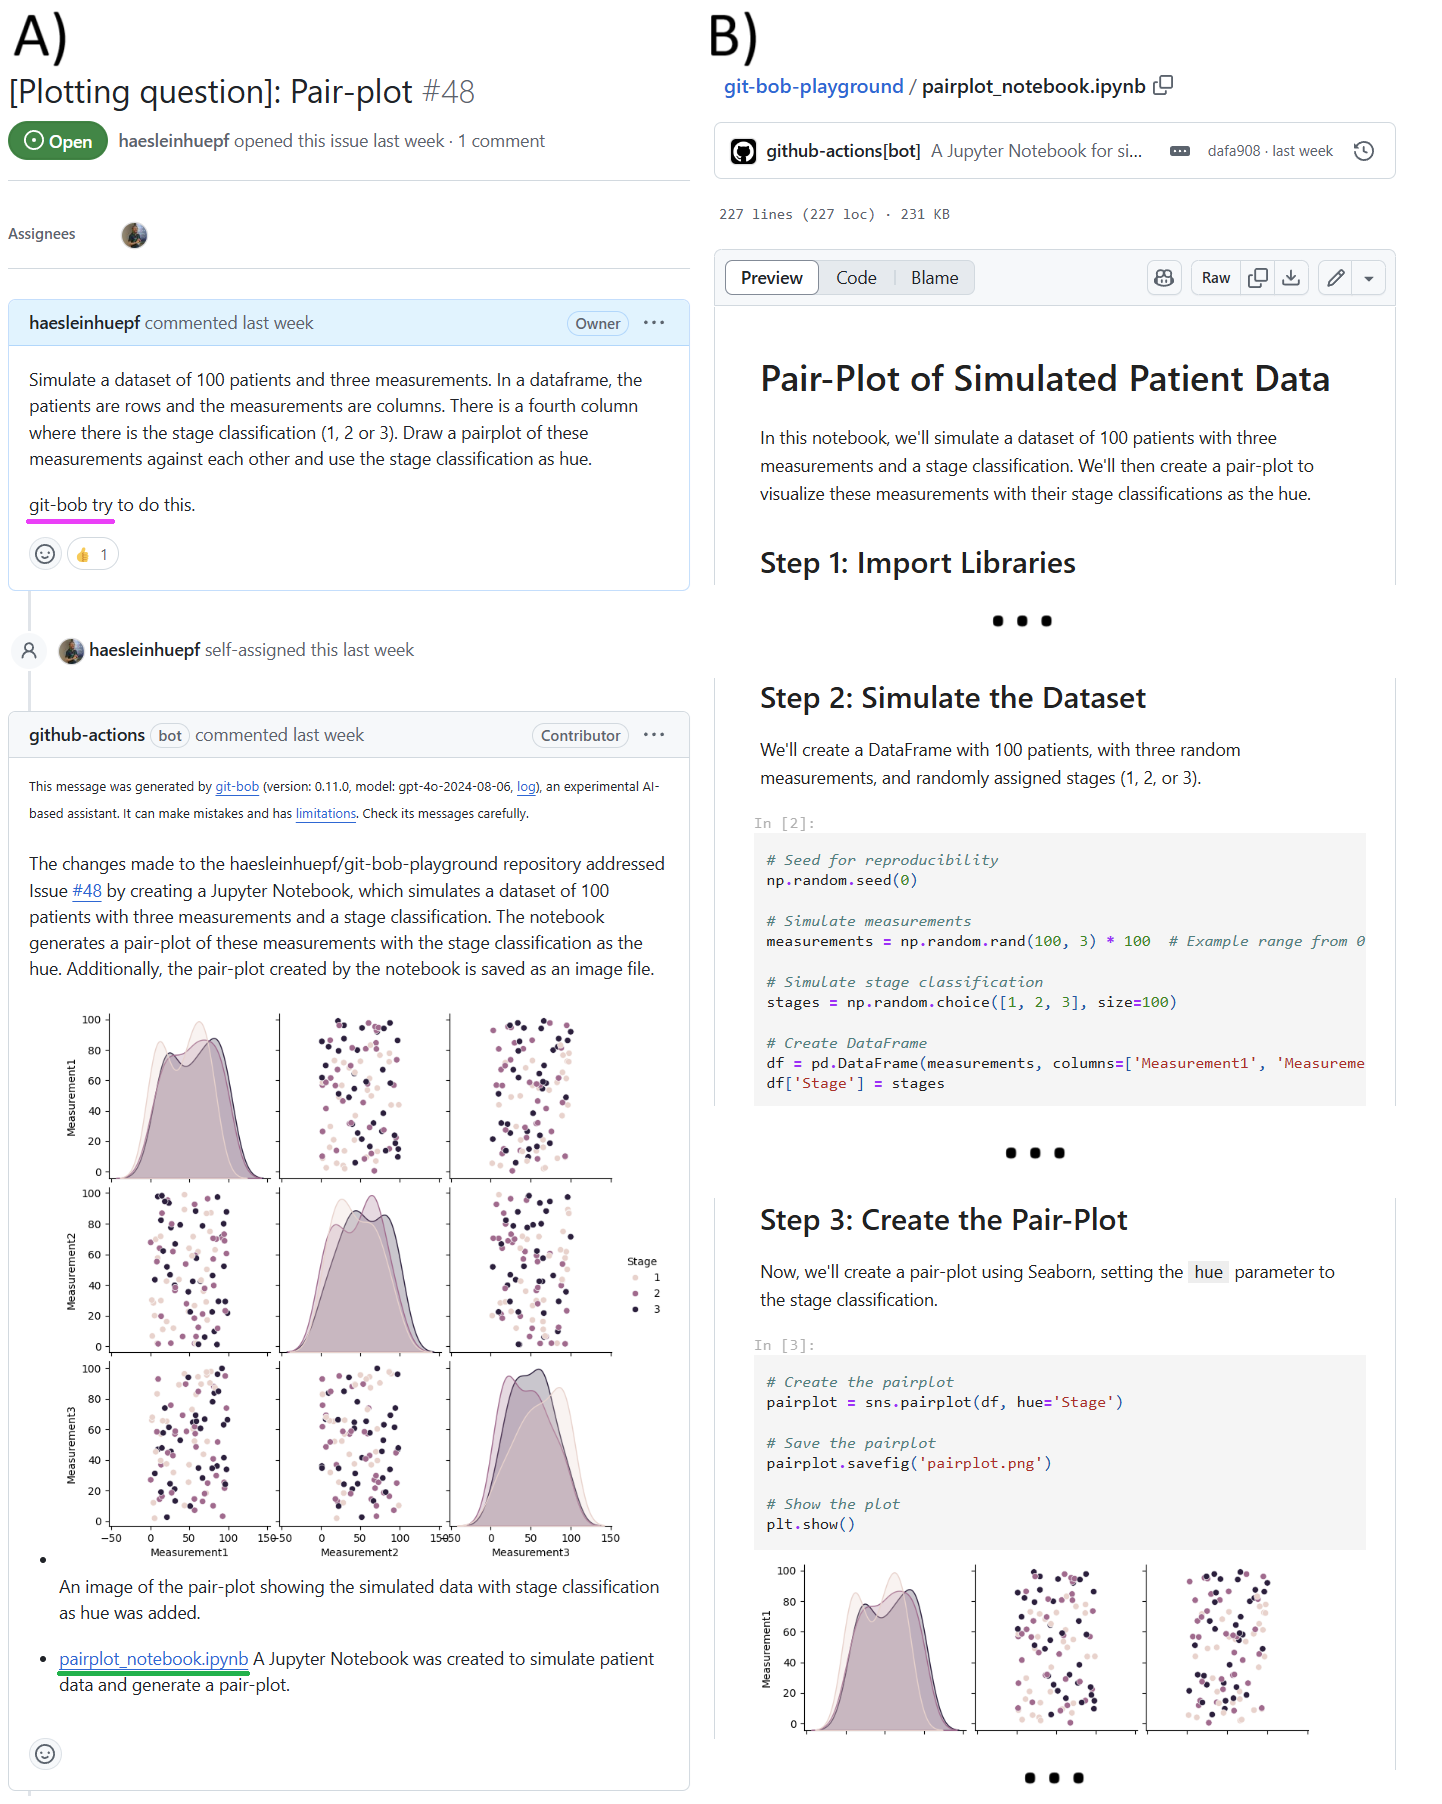
\includegraphics[width=0.9\textwidth]{example_pair_plot.png}
\caption{Use-case example for generating data analysis code: The user explains a scenario (A) and triggers git-bob (underlined in magenta). The AI-assistant generates and executes code and visualizes the resulting plot. The user can click on the link to the generated notebook (underlined in green) to go to the notebook (B) and read the code and see intermediate results. The shown notebook is an excerpt as indicated by ``...''. The entire discussion and corresponding code can be read online: \url{https://github.com/haesleinhuepf/git-bob-playground/issues/48}
\newline
\newline
}
\label{fig:examplepairplot}
\end{figure*}


\begin{figure*}[h]
\centering
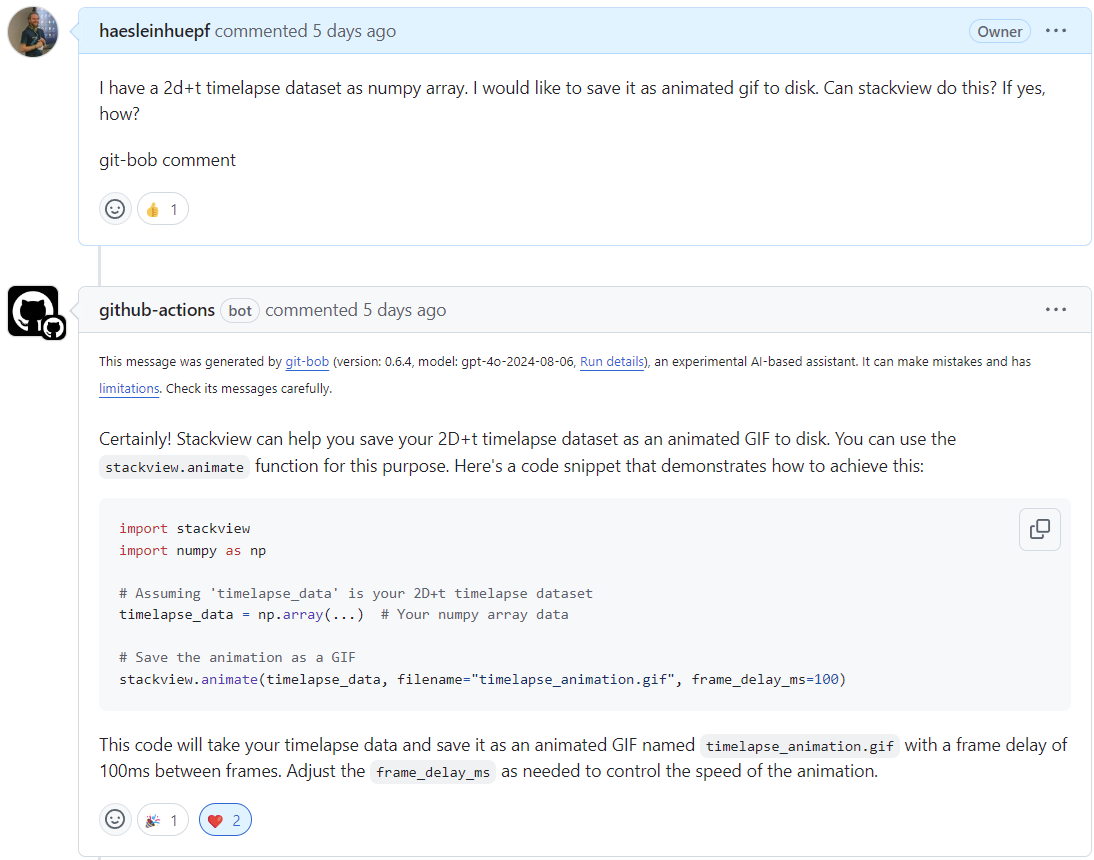
\includegraphics[width=0.8\textwidth]{example_supporting_users.png}
\caption{Use-case example for supporting users: The assistant can be configured to act as expert on a specific Python library and answer user questions. Words triggering git-bob are underlined in magenta. The entire discussion and corresponding code can be read online: \url{https://github.com/haesleinhuepf/stackview/issues/79}
\newline
\newline
}
\label{fig:examplesupportingusers}
\end{figure*}


\begin{figure*}[h]
\centering
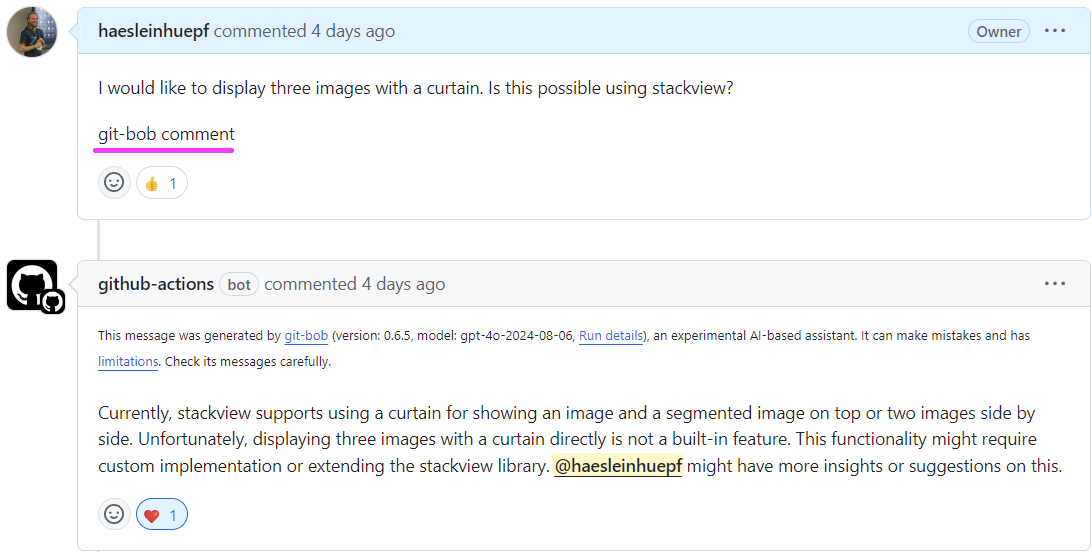
\includegraphics[width=0.8\textwidth]{example_supporting_users2.png}
\caption{Use-case example for asking an expert: The answer to the question shown here is "No", but this is nowhere written in the documentation or the configuration of the assistant. In this case the assistant is not sure, and it can be configured to forward a question to a maintainer of the library where the question arrived. Words triggering git-bob are underlined in magenta. The entire discussion and corresponding code can be read online: \url{https://github.com/haesleinhuepf/stackview/issues/80}
\newline
\newline
}
\label{fig:examplesupportingusers2}
\end{figure*}



\begin{figure*}[h]
\centering
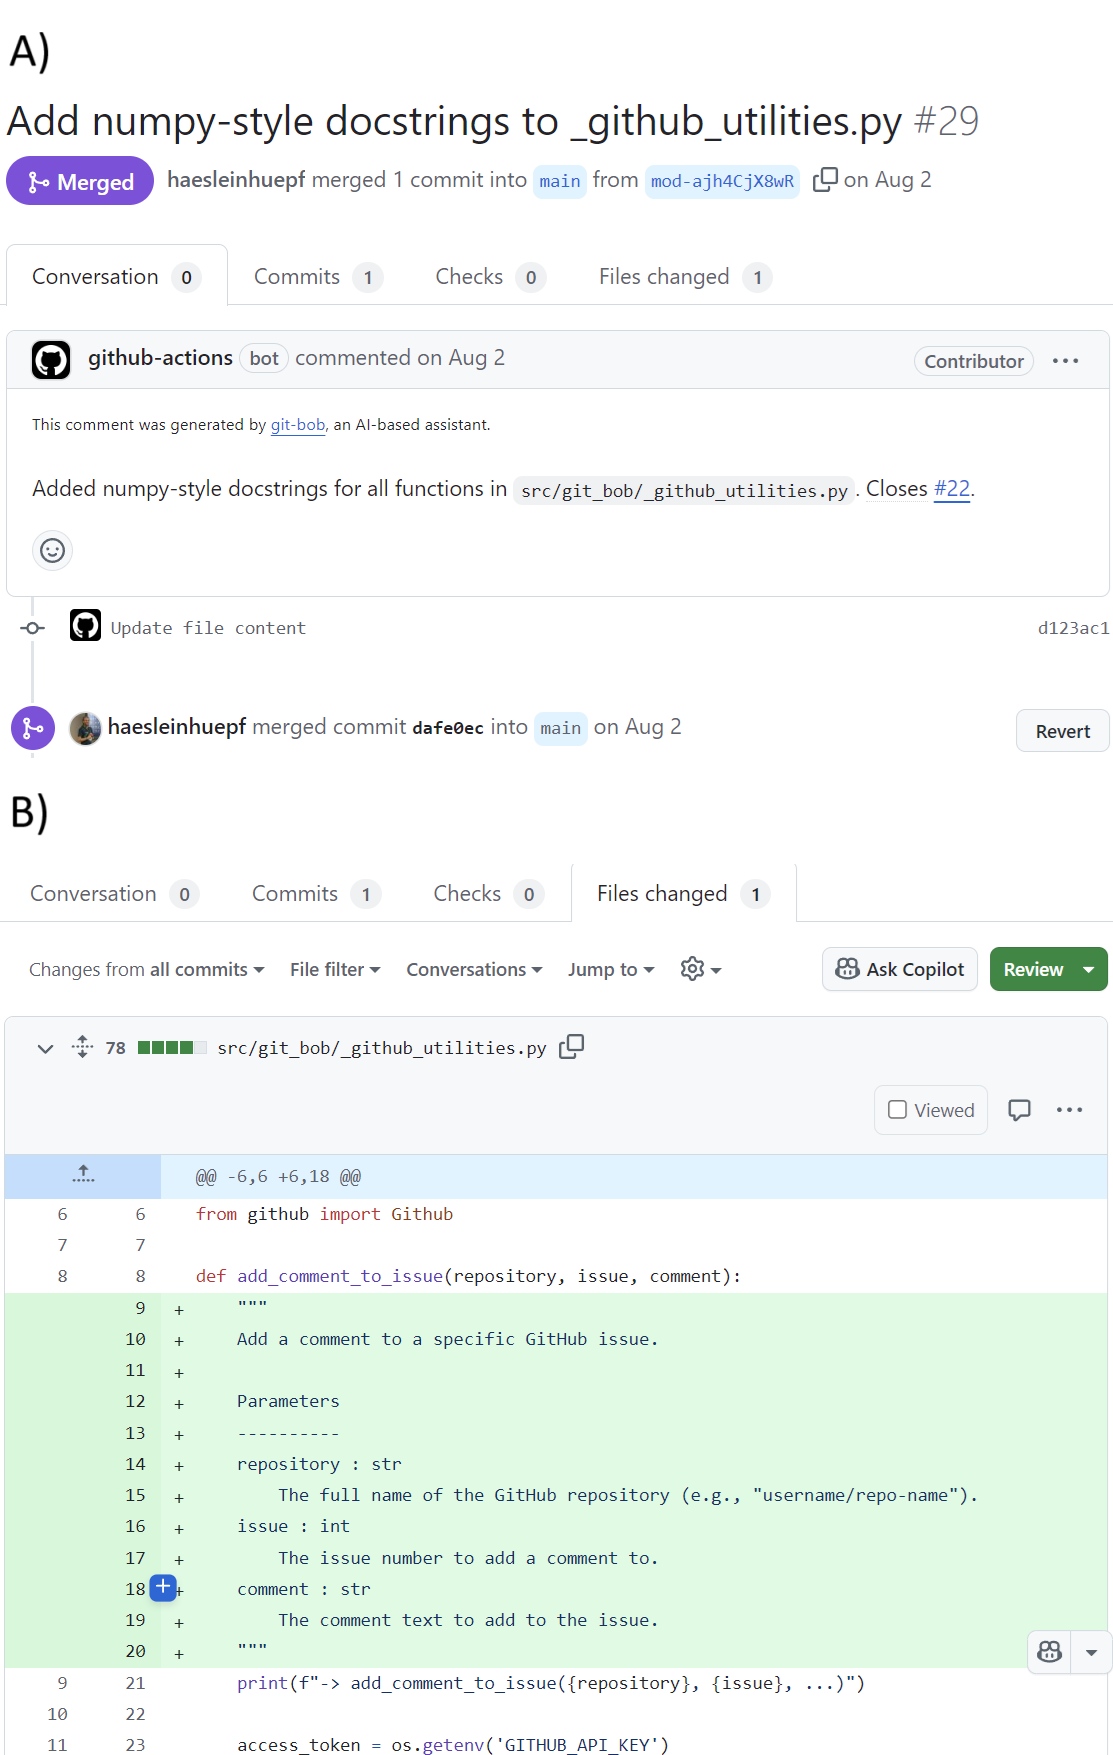
\includegraphics[width=0.82\textwidth]{example_add_documentation.png}
\caption{Use-case example for adding and revising documentation in code: git-bob was used to partially write the code documentation of its own code. When asked to add documentation in a specific format, it sent a pull-request (A) and the human could inspect the code modifications (B, excerpt) before mergin the code into the project's code base. The entire discussion and corresponding code can be read online: \url{https://github.com/haesleinhuepf/git-bob/pull/29}
\newline
\newline
}
\label{fig:example_add_documentation}
\end{figure*}


\begin{figure*}[h]
\centering
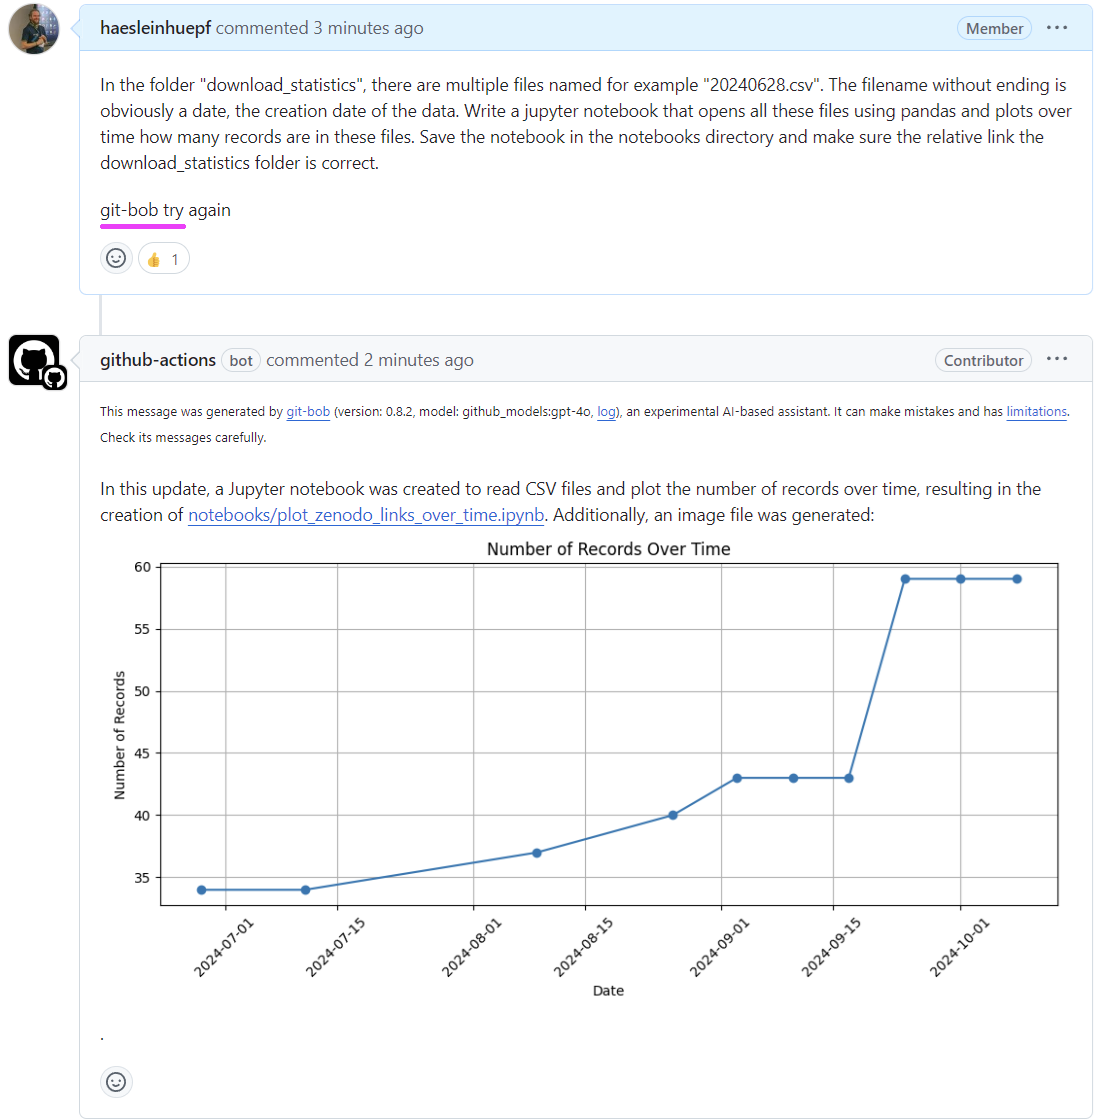
\includegraphics[width=\textwidth]{example_plotting.png}
\caption{Use-case example for plotting data: after explaining the assistant the folder structure of the project, it generates code for parsing a folder of CSV files and plotting results. Words triggering git-bob are underlined in magenta. The entire discussion and corresponding code can be read online: \url{https://github.com/NFDI4BIOIMAGE/training/issues/250}
\newline
\newline
}
\label{fig:exampleplotting}
\end{figure*}






\begin{figure*}[h]
\centering
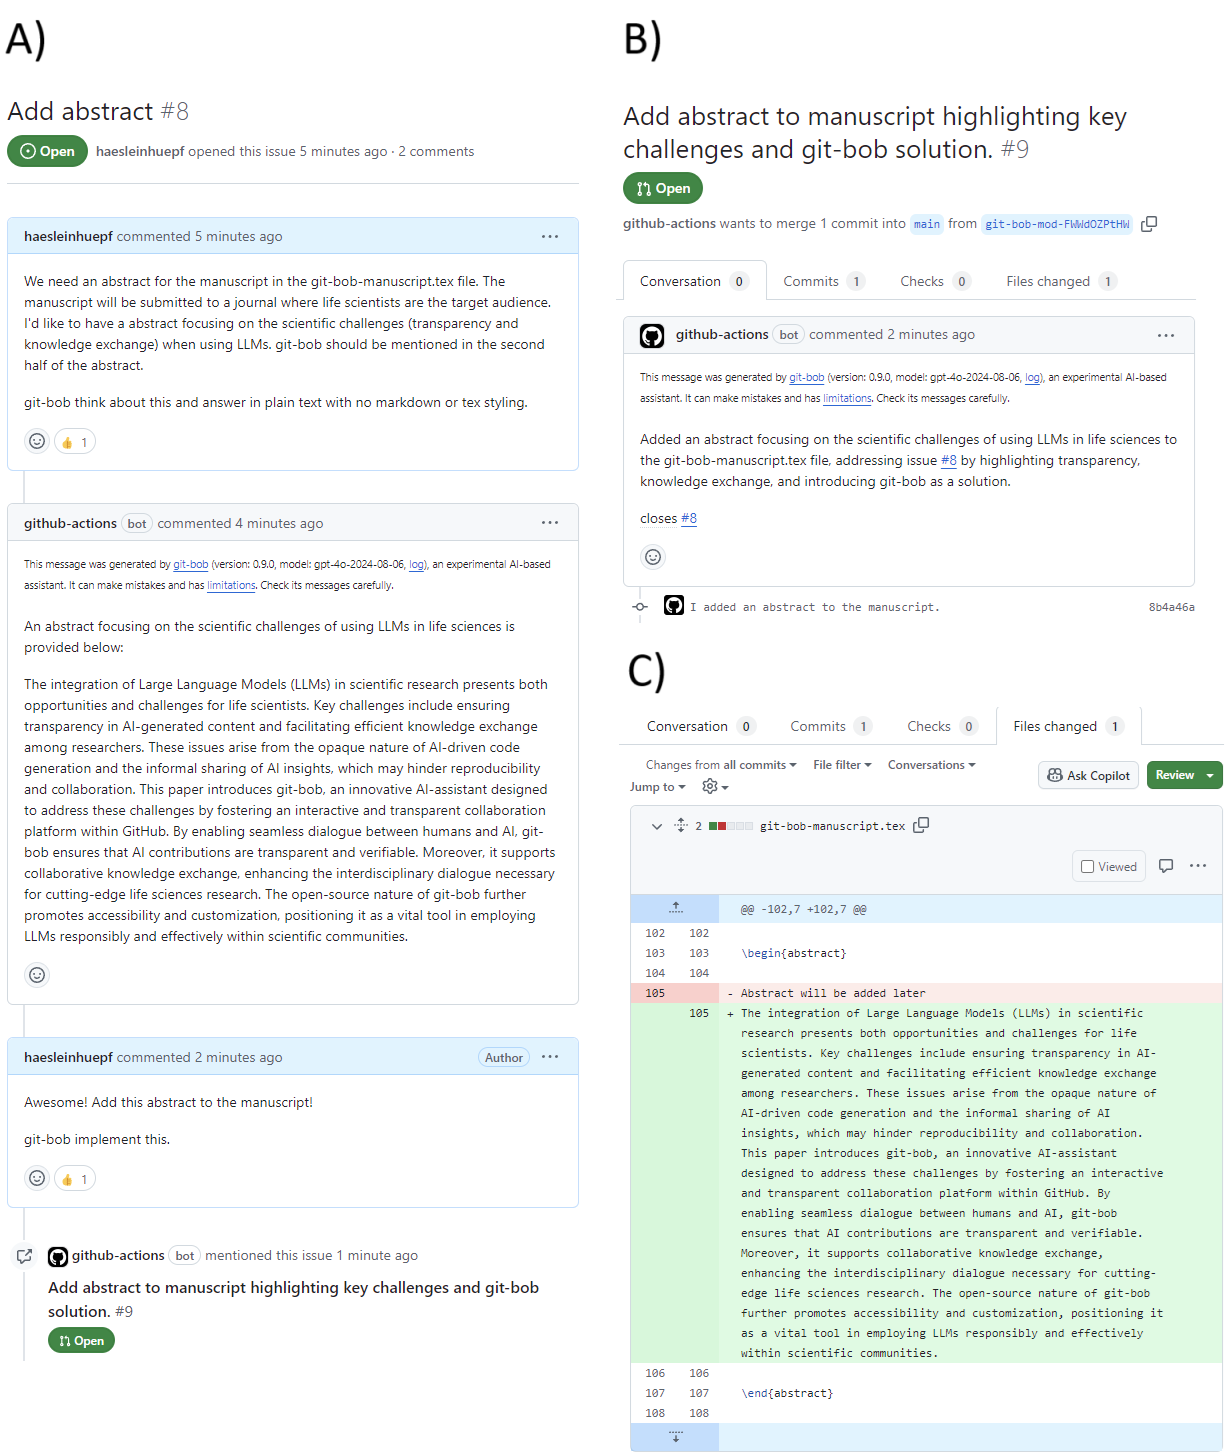
\includegraphics[width=\textwidth]{example_abstract_generation.png}
\caption{Use-case example for working on scientific manuscripts: after a first draft of the manuscript was written, git-bob was asked to formulate an abstract (A). The abstract was then submitted as pull-request with a short description (B). The human can also review and potentially modify the proposed text in this online interface (C). Words triggering git-bob are underlined in magenta. The entire discussion can be read online: \url{https://github.com/haesleinhuepf/git-bob-manuscript/issues/8} and \url{https://github.com/haesleinhuepf/git-bob-manuscript/pull/9}.
\newline
\newline
}
\label{fig:xample_abstract_generation}
\end{figure*}


%TC:endignore
%the command above ignores this section for word count

\end{document}
